% HW3 high dimensional data

\documentclass[12pt, leqno]{article}
\usepackage{amsfonts, amsmath, amssymb}
\usepackage{amsthm}
\usepackage{mathtools}
\usepackage{fancyhdr}
\usepackage{hyperref}
\usepackage{graphicx}
\usepackage{caption}
\usepackage{subcaption}
\usepackage{float}
\usepackage{mathrsfs}
\usepackage{array} 
\usepackage{rotating}
\usepackage{rotating}
\usepackage{booktabs}
\usepackage{bbm}
%\usepackage{babel}
\providecommand{\abs}[1]{\lvert#1\rvert}
\providecommand{\norm}[1]{\lVert#1\rVert}
\newcommand{\macheps}{\epsilon_{\mbox{\scriptsize mach}}}
\let\oldhat\hat
\renewcommand{\vec}[1]{\mathbf{#1}}
\renewcommand{\hat}[1]{\oldhat{{#1}}}
\def\rp{\ensuremath \mathbb{R}^p}
\def\rpp{\ensuremath \mathbb{R}^{p \times p}}
\def\s{\ensuremath\Sigma}
\def\om{\ensuremath\Omega}
\def\pd{\ensuremath\mathbb{P}^+}
\def\pg{\ensuremath\mathbb{P}_{{G}}}
\def\E{\ensuremath\mathbb{E}}
\def\normdist[#1]#2{\ensuremath \sim \mathcal{N} (#1,#2) }
\def\ndist1{\ensuremath \sim \mathcal{N}  (\mu, \sigma)}
\def\ndistvec{\ensuremath \sim \mathcal{N}_p ( {\mu},  {\Sigma})}
\def\lra{\ensuremath\Leftrightarrow}
\def\stackrel#1#2{\mathrel{\mathop{#2}\limits^{#1}}}
\newcommand\ind{\protect\mathpalette{\protect\independenT}{\perp}}
\def\independenT#1#2{\mathrel{\rlap{$#1#2$}\mkern2mu{#1#2}}}
\makeatletter
\newtheorem{thm}{Theorem}[]
\newtheorem{lemma}{Lemma}[]
\newtheorem{defn}[thm]{Definition}
\newcommand{\sign}{\mathrm{sign}}
\newcommand{\prox}{\mathrm{prox}}
\newcommand{\distas}[1]{\mathbin{\overset{#1}{\kern\z@\sim}}}%
\newsavebox{\mybox}\newsavebox{\mysim}
\newcommand{\dist}[1]{%
  \savebox{\mybox}{\hbox{\kern3pt$\scriptstyle#1$\kern3pt}}%
  \savebox{\mysim}{\hbox{$\sim$}}%
  \mathbin{\overset{#1}{\kern\z@\resizebox{\wd\mybox}{\ht\mysim}{$\sim$}}}%
}
\makeatother

\begin{document}
\pagestyle{fancy}
\lhead{Syed Rahman}
\rhead{STA7934}

\begin{center}
{\large {\bf Take Home Final - Analysis of High Dimensional Data}} \\
\end{center}

\paragraph{1a.} $f(x) = \norm{x}_1$ with domain of $f =
\{x:\norm{x}_{\infty} \leq 1\}$. 
Note that 
\begin{align*}
  [\prox_{f}(x)]_i &= \arg\min_{u}[(\norm{u}_1 + \frac{1}{2} \norm{u-x}_2^2)]_i\\
  &= \begin{cases} x_i-1 & \text{ if } x_i>1 \\
0 & \text{ if } \abs{x_i} \leq 1 \\
x_i + 1 & \text{ if } x_i<-1
\end{cases}
\end{align*}
Now for $\prox_{f}(x)$ such that $\{u:\norm{u}_{\infty} \leq 1\}$ we
have $\arg\min_{u} (\norm{u}_1 + \frac{1}{2} \norm{u-x}_2^2 + 
\norm{u}_{\infty})$. We can come up with an ADMM algorithm for this
using the constraint that $z = u$. Thus we have 
\begin{align*}
\arg\min \norm{u}_1 + \frac{1}{2} \norm{u-x}_2^2 + 
\norm{z}_{\infty} \text{ such that } z=u
\end{align*}
Then the augmented Lagrangain is 
\begin{align*}
  \mathcal{L}_{\rho}(u,z,\lambda) = \norm{u}_1 + \frac{1}{2} \norm{u-x}_2^2 + 
\norm{z}_{\infty} - \mu^T(z-u) + \frac{\rho}{2}\norm{z-u}_2^2
\end{align*}
Hence we have that 
\begin{align*}
u^{k+1} &= \arg\min_{u} \mathcal{L}_{\rho}(u,z^{k},\mu^{k}) \\
z^{k+1} &= \arg\min_{z} \mathcal{L}_{\rho}(u^{k+1},z,\mu^{k}) \\
\mu^{k+1} &= \mu^{k} + \rho(z-u)
\end{align*}
Now keeping everything other that $u$ fixed we have 
\begin{align*}
  \mathcal{L}_{\rho}(u,z,\mu) &= \norm{u}_1 + \frac{1}{2}
  \norm{u-x}_2^2 - \mu^T(z-u) + \frac{\rho}{2}\norm{z-u}_2^2
  \\
\implies \partial_u \mathcal{L}_{\rho}(u,z,\mu) &= s + (u-x) -
  \mu + \rho (u-z)
\end{align*}
where $s_i = \sign(u_i)$. Thus we can run a subgradient algorithm for
$u$. Now keeping everthing other than $z$ fixed we have 
\begin{align*}
  \mathcal{L}_{\rho}(u,z,\mu) &=
\norm{z}_{\infty} - \mu^T(z-u) + \frac{\rho}{2}\norm{z-u}_2^2
  \\
\implies \min_z \mathcal{L}_{\rho}(u,z,\mu) &= \min_z \frac{1}{2}
\norm{z}_{\infty} - \mu^Tz + \arg\min_z 
                                                      \frac{\rho}{2}\norm{z}_2^2
                                                      - {\rho} u^Tz
  \\
\implies \arg\min_z \mathcal{L}_{\rho}(u,z,\mu) &= \arg\max_{\mu
  \geq 0 }-\frac{1}{2}
  \norm{\mu}_1 + \arg\max_{\mu
  \geq 0 }-\frac{1}{2\rho}
  \norm{\mu-2\rho u}_2^2  \\
&= \arg\min_{\mu \geq 0} \frac{1}{2}
  \norm{\mu}_1 + \frac{1}{2\rho}
  \norm{\mu-2\rho u}_2^2
\end{align*}
Thus the $z$ update step is equivalent to solving a $lasso$ problem. 



\paragraph{1b.} $f(x) = \max_{k=1,...,n} x_k = \norm{x}_{\infty}$.
Thus 
\begin{align*}
\prox_{f} (x) &= \arg\min_{u} (\norm{u}_{\infty} +
               \frac{1}{2}\norm{u-x}_2^2) \\
\end{align*}
Note that
\begin{align*}
&\min_{u} \norm{u}_{\infty} +
               \frac{1}{2}\norm{u-x}_2^2\\
=& \min_{u} (\norm{u}_{\infty} - x^Tu) + \min_{u} \frac{1}{2} \norm{u}_2^2\\
\end{align*}
We can minimize the second part with respect to $u$ by taking
derivatives and getting that $u=0$.
Now $\arg\min_x \frac{1}{2} \norm{x}_1 + \frac{1}{2} \norm{x-u}_2^2 =
S_{1/2}(u)$, which implies that 
\begin{align*}
[S_{1/2}(u)]_i = \begin{cases} u_i-1/2 & \text{ if } u_i>1/2 \\
0 & \text{ if } \abs{u_i} \leq 1/2 \\
u_i + 1/2 & \text{ if } u_i<-1/2
\end{cases}
\end{align*}

\paragraph{2} We want to solve the following problem:
\begin{align*}
\textbf{Primal:}&\min (x_1 - x_2) \\
&\text{subject to } x \in X = \{x:x_1 \geq 0, x_2 \geq 0\}, x_1+1 \leq
  0, 1 - x_1 - x_2 \leq 0
\end{align*}
Now the Lagrangian is 
\begin{align*}
\mathcal{L}(x,\lambda) &= (x_1 - x_2) + \lambda_1(-x_1) +
                         \lambda_2(-x_2) \\
&\quad + \lambda_3(x_1+1) + \lambda_4(1 - x_1 - x_2) \\
&= x_1(1-\lambda_1+\lambda_3-\lambda_4) + x_2(-1 - \lambda_2 -
  \lambda_4) + \lambda_3 + \lambda_4 \\
\implies g(\lambda_1,\lambda_2,\lambda_3,\lambda_4) &=
                                                      \inf_{x}\mathcal{L}
                                                      (x,\lambda) \\
&= \begin{cases} -\infty & \text{ if } 1-\lambda_1+\lambda_3-\lambda_4
  \not= 0 \text { or } -1 - \lambda_2 -
  \lambda_4 \not= 0 \\
\lambda_3 + \lambda_4 & \text{ else }
\end{cases}
\end{align*}
Thus the dual problem is 
\begin{align*}
\textbf{Dual:}&\max_{\lambda_i \geq 0} \lambda_3 + \lambda_4 \\
&\text{subject to } 1-\lambda_1+\lambda_3-\lambda_4
  = 0 \\
& \text {and } -1 - \lambda_2 -
  \lambda_4 = 0
\end{align*}
The constraints have
infinitely many solutions. Hence this is clearly maximized when
$\lambda_i = \infty, i = 3,4$ which implies that the
dual is unbounded. 

\paragraph{3a.} Let $A_j \in \mathbb{R}^{m \times n}, y_j \in
\mathbb{R}$. We want to solve the following problem: 
\begin{align*}
\textbf{Primal:}&\min_{X \in \mathbb{R}^{m \times n}} \sum_{j = 1}^J
                  (y_j - tr(X'A_j))^2 \\
&\text{subject to } \norm{X}_* \leq t
\end{align*}
or equivalently,
\begin{align*}
\min_{X \in \mathbb{R}^{m \times n}} \sum_{j = 1}^J
                  (y_j - tr(X'A_j))^2 + \lambda \norm{X}_*
\end{align*} 
For our simulations we used, $m = 10,n = 5$ and $J = 5$. In addition,
$A_j$ are matrices with elements randomly generated from
$\mathcal{U}(-5,5)$. To generate the true $X$ we generated a matrix
with elements from $\mathcal{U}(-5,5)$ took the $SVD$ as $U \s V'$ and set
$X = UV'$. We then calculated $y_j =  tr(X'A_j) +
\epsilon_j$ where $\epsilon_j \sim \mathcal{N}(0,1)$. 
Note that $\frac{d}{dX} \sum_{j = 1}^J
                  (y_j - tr(X'A_j))^2 = -2 \sum_{j = 1}^J(y_j -
                  tr(X'A_j))A_j$.
Thus a proximal gradient method would be
\begin{align}
X^{k+1} &= X^{k} + t(2 \sum_{j = 1}^J(y_j -
                  tr((X^k)'A_j))A_j) \\
X^{k+1} &= S_{t\lambda}(X^{k+1})
\end{align}
where $t$ is the stepsize and $S_{t\lambda}(X^{k+1}) =
 U S_{t\lambda}(\s) V'$. Here, 
\begin{align*}
X &= U \s V' \\ 
&= U diag(\sigma_1,...,\sigma_p) V' 
\end{align*} 
is the SVD of $X$ and $S_{t\lambda}(\s) =
diag(S_{t\lambda}(\sigma_1),...,S_{t\lambda}(\sigma_p))$ is the soft
thresholding operator applied elementwise to the diagonal of $\s$.
Using a cross-validation procedure we find that $\lambda \approx 550$
minimizes the objective function as shown in Figure \ref{fig:no3cv}. Doing 10 replications using this
value of $\lambda$ converges in about $500-700$ iterations and gives
us an average Frobenius norm loss of
\[
F = \sum_{r = 1}^{10}\frac{\norm{\hat{X}_r-X_r}_F}{\norm{X_r}_F} =   0.9858716.
\]
\begin{figure}
\begin{center}
                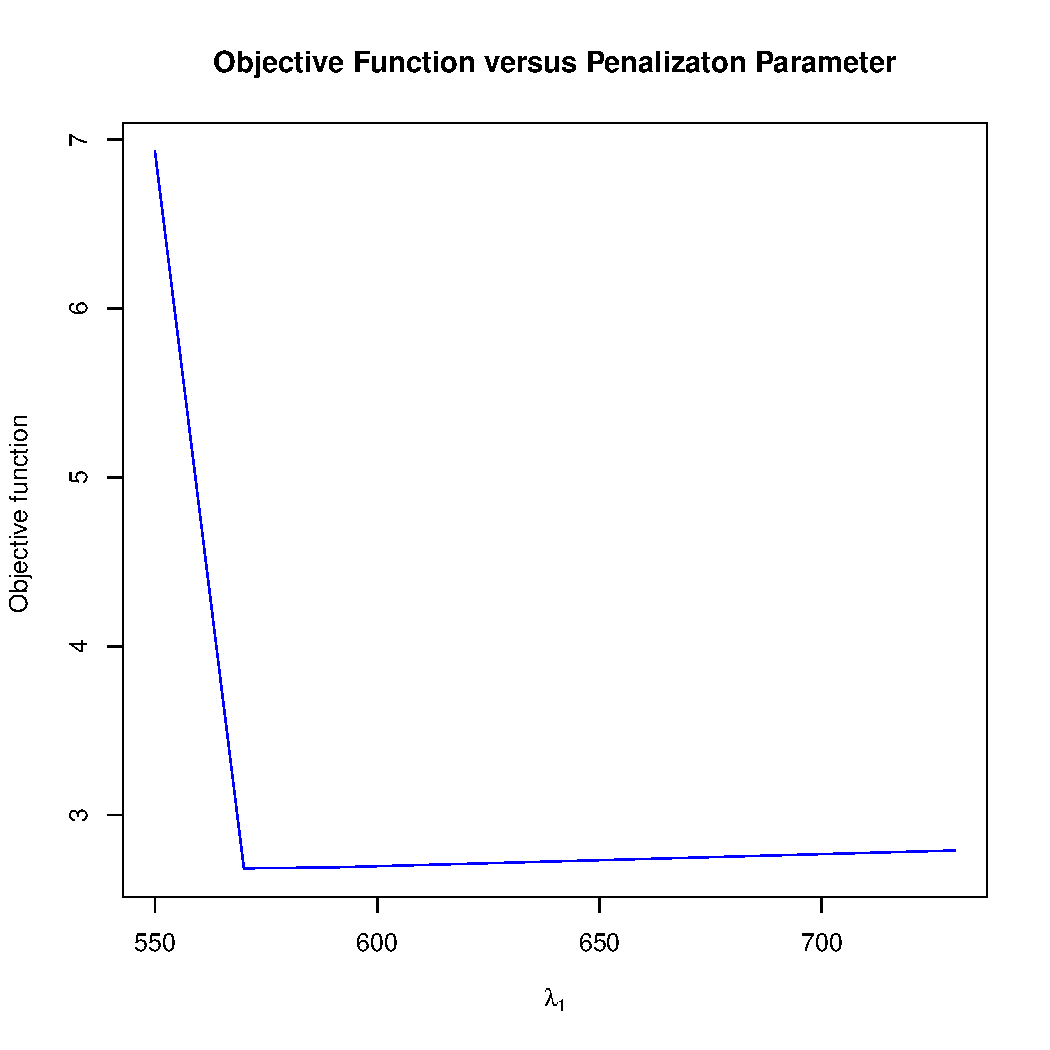
\includegraphics[scale = 0.5]{takehome3cv.pdf}
                \caption{Value of objective function for predicted $X_{\lambda}$ versus $\lambda$ for trace norm
                  constrained optimization problem}
                \label{fig:no3cv}
\end{center}
\end{figure}

\paragraph{4.}
For the second method we want to solve the following problem for $i = 1,...,p$:
\begin{align*} \textbf{Method 2:}
&\min \norm{\beta^{1}}_1 + \norm{\beta^{2}}_1 \\
&\text{subject to } \norm{S\beta^{1} - e_i}_{\infty} \leq t_1 ,
  \norm{S\beta^{2} - e_i}_{\infty} \leq t_2 \\
&\text{ and } \norm{\beta^{2} - \beta^{1}}_{\infty} \leq t_3
\end{align*}
Note that this is equivalent to
\begin{align*}
&\min \norm{\beta^{1}}_1 + \norm{\beta^{2}}_1 \\
&\text{subject to } - t_11 \leq S\beta^{1} - e_i\leq t_11 \\
&\text{and }  -t_21 \leq S\beta^{2} - e_i \leq t_21 \\
&\text{ and } -t_31 \leq \beta^{2} - \beta^{1} \leq t_31
\end{align*}
Now reparametrize by letting $u^1 = \abs{\beta^{1}}_1$ and $u^2 =
\abs{\beta^{2}}_1$. Then the problem is 
\begin{align*}
&\min \sum_{j = 1}^p{u_j^1} +  \sum_{j = 1}^p{u_j^2} \\
&\text{subject to } -\beta^{1} \leq u^1 \leq \beta^{1},-\beta^{2} \leq
  u^2 \leq \beta^{2} \\
&\text{ and } - t_11 \leq S\beta^{1} - e_i\leq t_11 \\
&\text{and }  -t_21 \leq S\beta^{2} - e_i \leq t_21 \\
&\text{ and } -t_31 \leq \beta^{2} - \beta^{1} \leq t_31
\end{align*}
or equivalently,
\begin{align*}
&\min \sum_{j = 1}^p{u_j^1} +  \sum_{j = 1}^p{u_j^2} \\
&\text{subject to } 0 \leq 2u^1 + (\beta^{1}-u^1) \leq 2 \beta^{1},0 \leq 2u^2+
  (\beta^{2}-u^2) \leq 2\beta^{2} \\
&\text{ and } S(\beta^{1} + u^1) - Su^1\leq e_i + t_11 \\
&\text{ and }  - (S(\beta^{1} + u^1) - Su^1)  \leq t_11 - e_i \\
&\text{ and } S(\beta^{2} + u^2) - Su^2 \leq e_i + t_21 \\
&\text{ and }  - (S(\beta^{2} + u^2) - Su^2)  \leq t_21 - e_i \\
&\text{ and } (\beta^{1} - u^1) - (\beta^{2} - u^2) + u^1 - u^2 \leq -t_31 \\
&\text{ and } (\beta^{2}-u^2)- (\beta^{1}-u^1) - u^1 + u^2\leq t_31 \\
\end{align*}
Hence we can write the above problem as a linear programming problem:
\begin{align*}
&\min c^Tx \\
&\text{subject to } Ax \leq b \\
&\text{and } x \geq 0
\end{align*}
where 
\[
x = \begin{pmatrix} u^1 \\u^2 \\\beta^{1} + u^1 \\ \beta^{2} + u^2 \end{pmatrix},
\]
\[
c^T = \begin{pmatrix} 1 &1&0&0 \end{pmatrix},
\]
\[
A = \begin{pmatrix} 
-2I&0&I&0\\
0&0&-I&0\\
0&-2I&0&I\\
0&0&0&-I\\
-S&0&S&0\\
S&0&-S&0\\
0&-S&0&S\\
0&S&0&-S\\
I&-I&-I&I\\
-I&I&I&-I\\
\end{pmatrix},
\]
and
\[
b^T = \begin{pmatrix}
  0&0&0&0&t_11+e_i&t_11-e_i&t_21+e_i&t_21-e_i&t_31&-t_31 \end{pmatrix}.
\]
Then set $\hat{B}^1 = (\hat{B}^1+\hat{u}^1) - \hat{u}^1$ and
$\hat{B}^2 = (\hat{B}^2+\hat{u}^2) - \hat{u}^2$ and let the solutions
to the $i$-th problem be the $i$-th columns of
$\hat{\om}^1$ and $\hat{\om}^2$. 

\begin{table}[H]
\begin{center}
\resizebox{0.9\textwidth}{!}{\begin{minipage}{\textwidth}
\begin{center}
\begin{tabular}{r|c|c|c}
\toprule
&Chain&{Nearest Neighbor
        }&{Scale-free }\\
\midrule
$F$&0.1221728&0.08730594&134.422\\  
$F_{mle}$&0.02973216&0.1672218&185.1804\\  
$FP$&0.1242754&0.3097686&0.1264815\\   
$FN$&0&0.3822743&0.3216667\\         
\bottomrule
\end{tabular}
\caption[]{
A comparison of the Dantzig Selector Joint estimation method for Chain,
  Nearest Neighbor network and Scale-free network graphs.
  For the chain graph, the prediction of the
sparsity pattern and estimation of the concentration matrix tends to be very accurate than for the Nearest
Neighbor Network and the Scale-Free Network as is
indicated by the higher values. Frobenius Norm Loss is especially poor
for the Scale-free Network.}
\label{tab:compare}
\end{center}
\end{minipage} }
\end{center}
\end{table}

\end{document}